\documentclass[11pt]{article}
\usepackage{graphicx}
\usepackage[margin=2.5cm]{geometry}
\usepackage{tikz}
\usepackage{indentfirst}
\usepackage{tabularx}
\usepackage{listingsutf8}
\usepackage{color}
\usepackage{hyperref}
\usepackage[portuguese]{babel}

\graphicspath{{./images/}}

\lstset{
	belowcaptionskip=1\baselineskip,
	captionpos=b,
	frame=tb,
	language=c,
	aboveskip=3mm,
	belowskip=3mm,
	showstringspaces=false,
	columns=flexible,
	basicstyle={\small\ttfamily},
	numbers=none,
	numberstyle=\tiny\color{gray},
	keywordstyle=\color{blue},
	commentstyle=\color{dkgreen},
	stringstyle=\color{mauve},
	breaklines=true,
	breakatwhitespace=true,
	tabsize=3,
	inputencoding=utf8,
	extendedchars=true,
	literate={á}{{\'a}}1 {ã}{{\~a}}1 {à}{{\`a} }1 {Ã}{{\~A}}1 {ó}{{\'o}}1 {Ó}{{\'O}}1 {Í}{{\'I}}1 {í}{{\'i}}1 {é}{{\'e}}1 {ç}{{\c{c}}}1 {Ç}{{\c{C}}}1 {ú}{{\'u}}1 {õ}{{\~o}}1
}

\begin{document}
	\begin{titlepage}
    	\begin{center}
    		
\includegraphics[width=0.6\textwidth]{logo-isec}
    		
    		\vspace*{\fill}
    		
    		\Huge
    		\textbf{Encaminhamento de Dados}
    		
    		\huge
    		Projeto de planeamento e configuração de uma rede
    		
    		\vspace{0.5cm}
    		\LARGE
    		2020 - 2021
    		
    		\vspace{1.5cm}
    		
    		\textbf{Bruno Teixeira - 2019100036}
    		
    		\vfill
    		\vspace*{\fill}
    		
    		\normalsize
    		Licenciatura em Engenharia Informática \\
    		18 de junho de 2021		
    	\end{center}
    \end{titlepage}
	


	\tableofcontents
	\pagebreak
	\listoffigures
	\pagebreak
	
	\large	
	\section{Introdução}
	\normalsize
	\paragraph{}
	Este trabalho tem como objetivo o planeamento de uma rede de dados alargada e distríbuida de uma organização fictícia com o intuito de alargar a competência do aluno no que toca a planeamento do projeto, desenho e implementação de redes locais e alargadas e respetiva configuração de routers baseados no sistema operativo Cisco IOS/IOU.    
    
	\large
	\section{Topologia}
	\normalsize
	
	\begin{figure}[h]
		\centering
		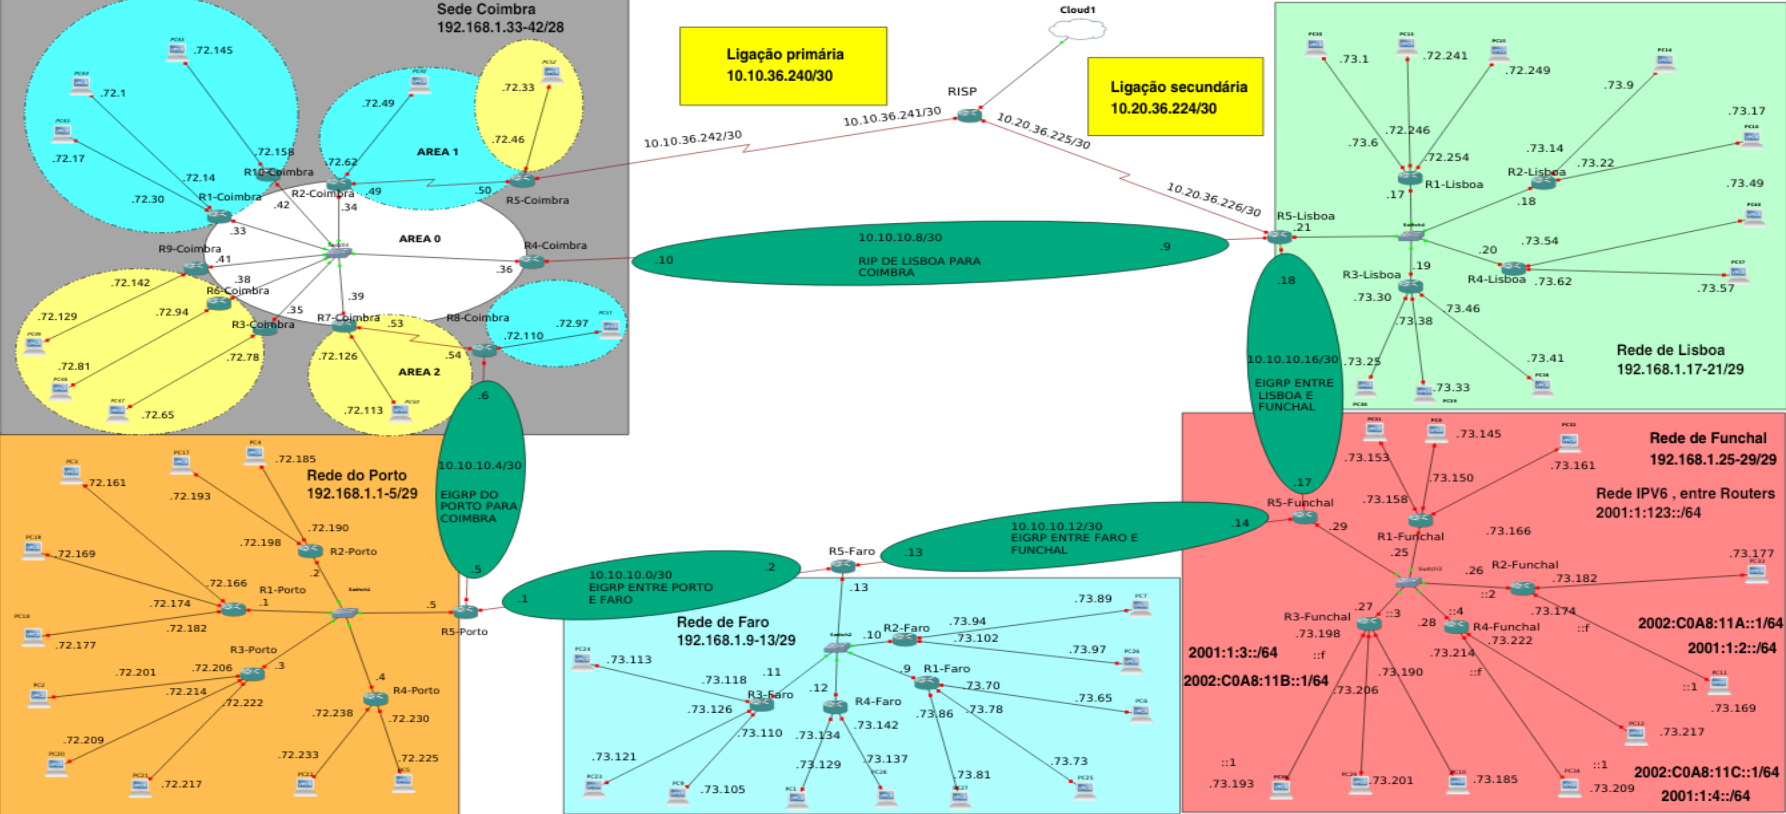
\includegraphics[width=1\textwidth]{topologia}
		\caption{Topologia}
		\label{fig.nav}
	\end{figure}
	
	\large
	\section{Endereçamento}
	\subsection{Endereçamento privado}
	\normalsize
    \paragraph{}

    Para o endereçamento privado foi usada a gama \textbf{192.168.1.0/29}(filiais) e \textbf{192.168.1.0/28}(sede) para a ligação entre routers dentro da mesma filial. \\
    Para o endereçamento privado entre routers de saída de filiais foi usado o \textbf{10.10.10.0/30}.

    \begin{figure}[h]
		\centering
		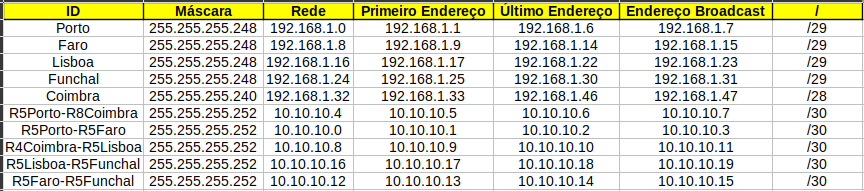
\includegraphics[width=0.6\textwidth]{privado}
		\caption{Endereçamento Privado}
		\label{fig.nav}
	\end{figure}

	\subsection{Endereçamento público}
	\normalsize
	\paragraph{}
    
    Foi usado VLSM no endereçamento público, fazendo com que cada \emph{link} de cada router representasse uma subrede diferente. A máscara usada no VLSM de cada filial é sempre igual, ou seja ,\textbf{/29}, no entanto em Coimbra, uma vez que é a sede, foi usado o \textbf{/28}.

    O endereçamento atribuido pelo ISP foi o \textbf{194.65.72.0} e o \textbf{194.65.73.0}.
    
	
	\large
	\section{Filiais}
	\normalsize
	\paragraph{}
	Todos os protocolos pedidos no enunciado foram usados nas filiais com a devida autenticação, assim como tambem foram mudadas as larguras de banda de cada \emph{link}. Todos os routers contêm uma única autenticação por \textbf{telnet} e é apresentado um \textbf{banner} aquando da entrada no mesmo. Prestou-se especial atenção para as rotas que não faziam sentido, ou seja, todas as subredes que saiam de uma filial para outra vão sempre pelo caminho mais eficiente não dando saltos desnecessários.

	\begin{figure}[h]
		\centering
		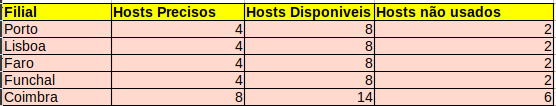
\includegraphics[width=0.6\textwidth]{redes-pub}
		\caption{Tabela para o endereçamento público das filiais}
		\label{fig.nav}
	\end{figure}
	
	\subsection{Coimbra}
	\normalsize
	\paragraph{}
	Em Coimbra foi usado o protocolo \textbf{OSPF} com a intenção de haver várias áreas.
	Uma vez que existiam áreas que não estavam ligadas à area 0, foi preciso fazer links virtuais, links estes que tambem contêm autenticação.\\
	
	No \textbf{R3-Coimbra} foi criada a \textbf{área 2} como sendo uma área \textbf{stub} de modo a que fosse possível receber rotas de outras áreas (\textbf{O IA}) e não fosse permitido propagar rotas externas nos dois sentidos. \\

	Existe uma ligação primária, ligação esta que parte do \textbf{R5-Coimbra} para o \textbf{RISP} em que foi usado o comando \emph{default-information originate metric-type 1} indicando que este é o router de saída e que as rotas são do tipo 1. No \textbf{R4-Coimbra} tambem foi definido o comando \emph{default-information originate} caso a saída primária esteja desligada, todo o trafégo sai pelo \textbf{R4-Coimbra}.

	\begin{figure}[h]
		\centering
		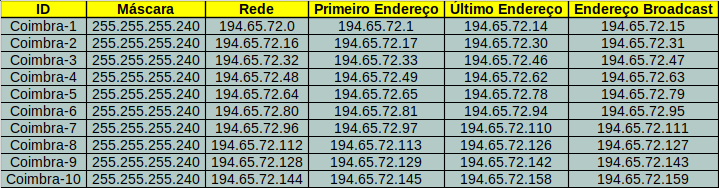
\includegraphics[width=0.6\textwidth]{vlsm-coimbra}
		\caption{VLSM de Coimbra}
		\label{fig.nav}
	\end{figure}

	\pagebreak

	\subsection{Porto}
	\normalsize
	\paragraph{}
	No Porto foi usado o protocolo \textbf{EIGRP} conforme pedido no enunciado.A sumarização foi desligada porque estavamos presentes numa rede \textbf{não contígua} e, mesmo o \textbf{EIGRP} tendo atenção à má sumarização de rotas, o melhor foi desligar. Por causa disto foram introduzidas \emph{discard routes} manuais para que a tabela de \emph{routing} ficasse com a informação correta.

	\begin{figure}[h]
		\centering
		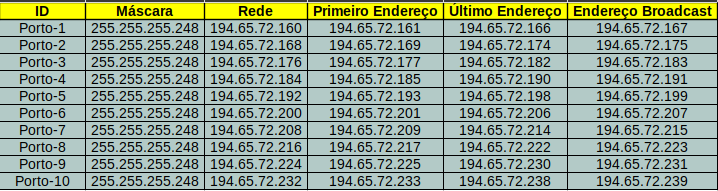
\includegraphics[width=0.6\textwidth]{vlsm-porto}
		\caption{VLSM do Porto}
		\label{fig.nav}
	\end{figure}

	\subsection{Lisboa}
	\normalsize
	\paragraph{}
	Em Lisboa foi usado o protocolo \textbf{RIP} usando a versão 2 para "transformar" o \textbf{RIP} num protocolo \emph{classless} de modo a podermos usar VLSM e o mesmo perceber. Aqui existe uma ligação secundária fazendo com que esta fique ativa caso a saída primária esteja em baixo. Para isto, no \textbf{RISP} usou-se uma métrica maior para a rota de saída para Lisboa e em Lisboa foi criada uma \emph{default route} com métrica de 125 fazendo com que esta seja a rota secundária. 

	Em Lisboa era tambem pedido que fosse criada uma \emph{prefix list} para que um router não recebesse rotas RIP vindas de um router qualquer dentro da filial. Então para isso foi criada uma \emph{prefix list} no \textbf{R3-Coimbra} de modo a que não fosse possível receber mensagens RIP vindas do \textbf{R4-Coimbra}.

	\begin{lstlisting}
		ip prefix-list NEGA1_R4-LISBOA deny 194.65.73.48/29
		ip prefix-list NEGA1_R4-LISBOA deny 194.65.73.56/29
		ip prefix-list NEGA1_R4-LISBOA permit 0.0.0.0/0 le 32
		router rip ... distribute-list prefix NEGA1_R4-LISBOA in e0/0
	\end{lstlisting}

	\begin{figure}[h]
		\centering
		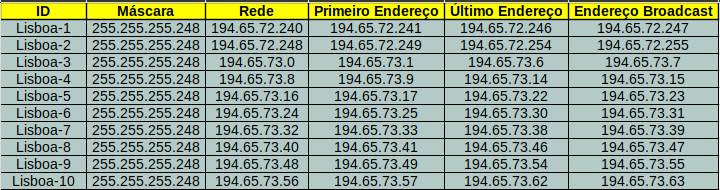
\includegraphics[width=0.8\textwidth]{vlsm-lisboa}
		\caption{VLSM de Lisboa}
		\label{fig.nav}
	\end{figure}


	\subsection{Funchal}
	\normalsize
	\paragraph{}
	No Funchal foi usado o \textbf{IPv6} com túneis dinâmicos em três subredes assim como o protocolo \textbf{EIGRP}, protocolo este que tanto foi usado no \textbf{IPv6} como no \textbf{IPv4}. Mais uma vez aqui a sumarização do \textbf{EIGRP} está desligada, tendo então colocado \emph{discard routes} manualmente.

	\begin{figure}[h]
		\centering
		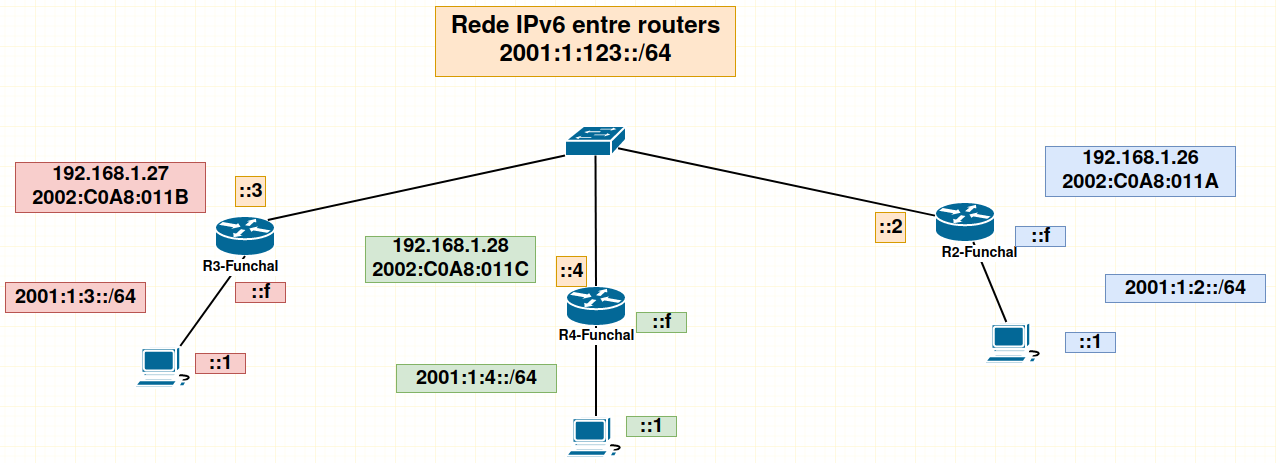
\includegraphics[width=0.8\textwidth]{ipv6}
		\caption{Planeamento IPv6}
		\label{fig.nav}
	\end{figure}

	\begin{figure}[h]
		\centering
		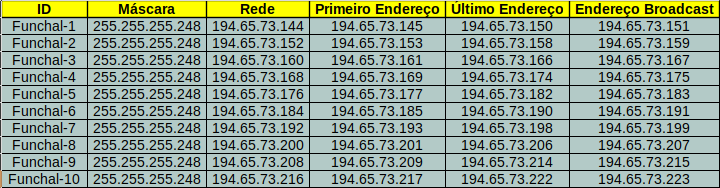
\includegraphics[width=0.8\textwidth]{vlsm-funchal}
		\caption{VLSM do Funchal}
		\label{fig.nav}
	\end{figure}


	\subsection{Faro}
	\normalsize
	\paragraph{}
	A escolha de protocolo em Faro era livre, logo optei por usar o \textbf{EIGRP} uma vez que é extremamente simples de o configurar. Mais uma vez, a sumarização do mesmo está desligada e foram feitas \emph{discard routes} manuais.

	\begin{figure}[h]
		\centering
		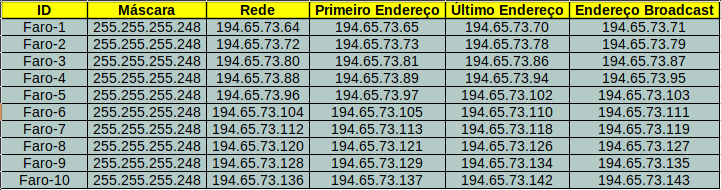
\includegraphics[width=0.8\textwidth]{vlsm-faro}
		\caption{VLSM de Faro}
		\label{fig.nav}
	\end{figure}

	\subsection{Comunicação entre filiais}
	\normalsize
	\paragraph{}
	Entre filiais foram redistribuidos alguns protocolos, fazendo com que um router conseguisse "traduzir" de um protocolo para o outro. De Coimbra (\textbf{R4-Coimbra}) para Lisboa (\textbf{R5-Lisboa}) foi usado o \textbf{RIPv2} redistribuindo de Lisboa para Coimbra. De Coimbra (\textbf{R8-Coimbra}) para o Porto (\textbf{R5-Porto}) foi redistribuido o \textbf{EIGRP} do Porto para Coimbra. \\
	Entre Porto (\textbf{R5-Porto}) e Faro (\textbf{R5-Faro}) foi usado o \textbf{EIGRP} assim como de Faro (\textbf{R5-Faro}) para o Funchal (\textbf{R5-Funchal}) e como do Funchal (\textbf{R5-Funchal}) para Lisboa (\textbf{R5-Lisboa}).    
	
	\large	
	\section{Saída primária e secundária}
	\normalsize
	\paragraph{}
	Na primeira imagem em baixo encontra-se um exemplo de uma tabela de \emph{routing} em que mostra algumas rotas assim como a \emph{default route} tendo a saída primária ligada. No segundo exemplo é mostrada a tabela de \emph{routing} do mesmo router (\textbf{R2-Coimbra}) mas desta vez com a saída primária desligada, ou seja, fazendo referência à saída secundária que se encontra em Lisboa. 

	\begin{figure}[h]
		\centering
		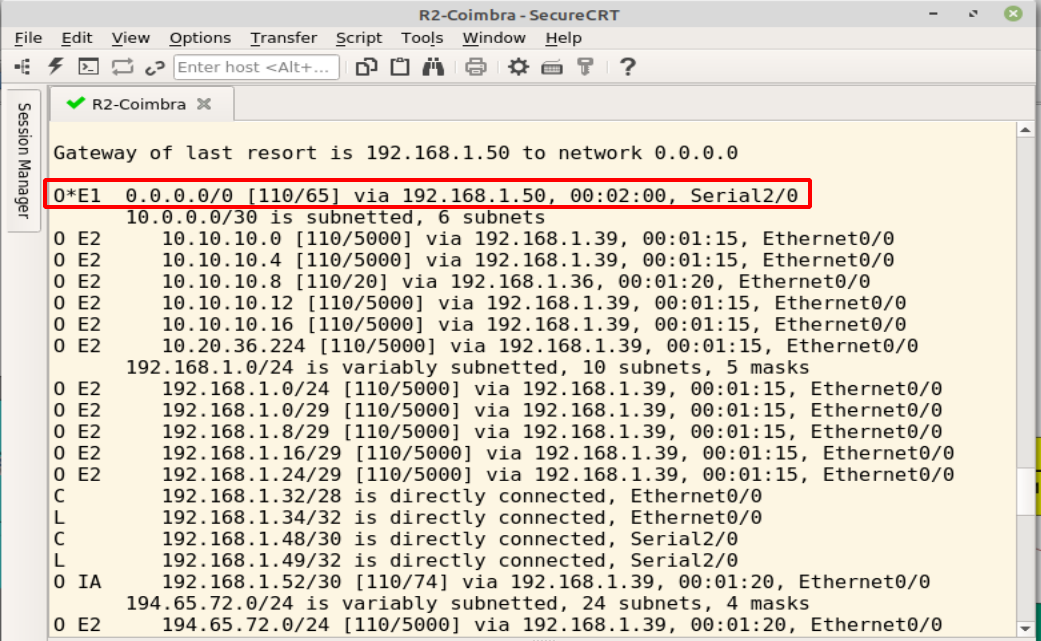
\includegraphics[width=0.6\textwidth]{saida-primaria}
		\caption{Saída primária pelo R5-Coimbra}
		\label{fig.nav}
	\end{figure}


	\begin{figure}[h]
		\centering
		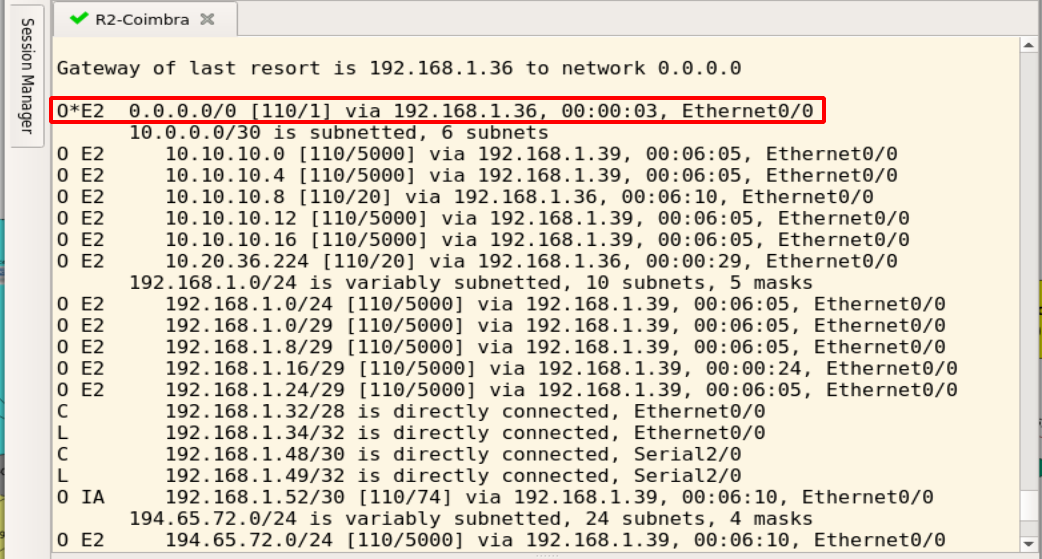
\includegraphics[width=0.6\textwidth]{saida-secundaria}
		\caption{Saída secundária pelo R5-Lisboa}
		\label{fig.nav}
	\end{figure}

	\pagebreak

	\large	
	\section{Tabelas de \emph{routing}}
	\normalsize

	\begin{figure}[h]
		\centering
		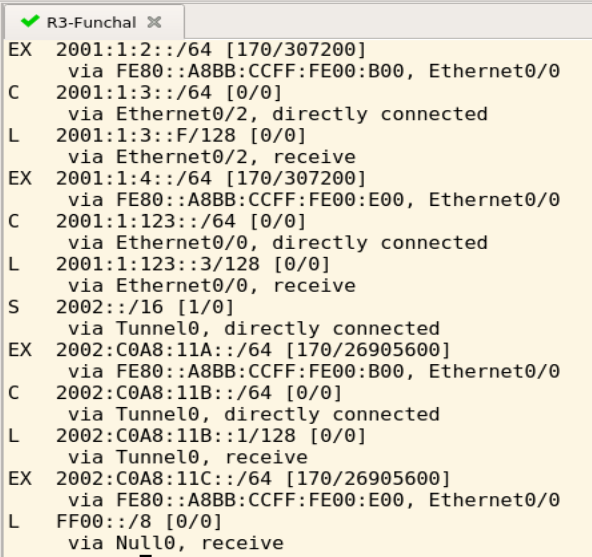
\includegraphics[width=0.4\textwidth]{routing-funchal}
		\caption{Excerto da tabela de \emph{routing} do Funchal}
		\label{fig.nav}
	\end{figure}

	\begin{figure}[h]
		\centering
		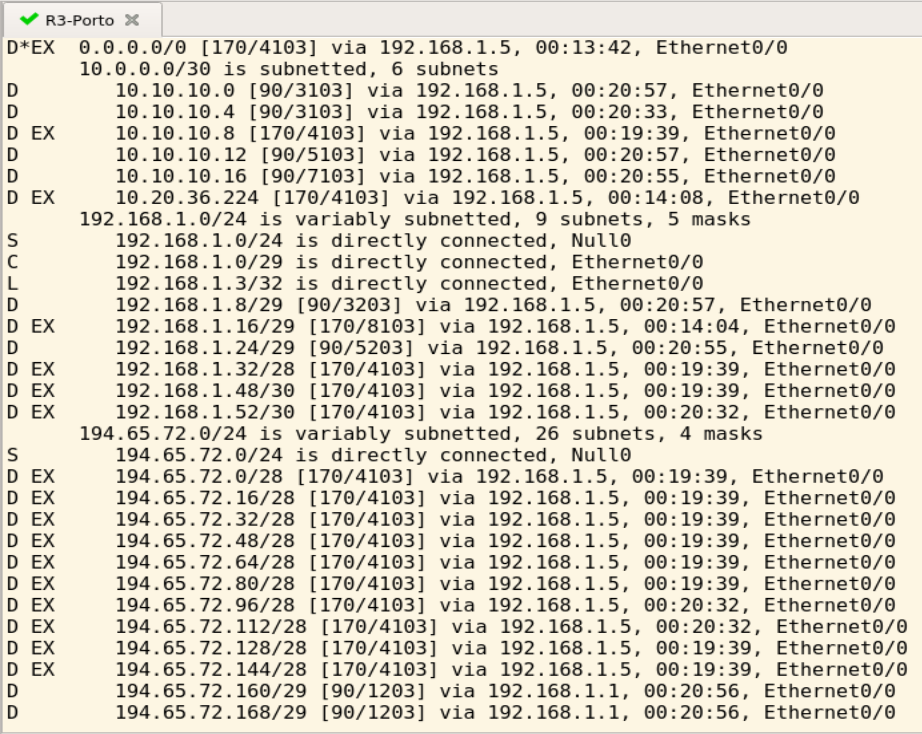
\includegraphics[width=0.6\textwidth]{routing-porto}
		\caption{Excerto da tabela de \emph{routing} do Porto}
		\label{fig.nav}
	\end{figure}

	\begin{figure}[h]
		\centering
		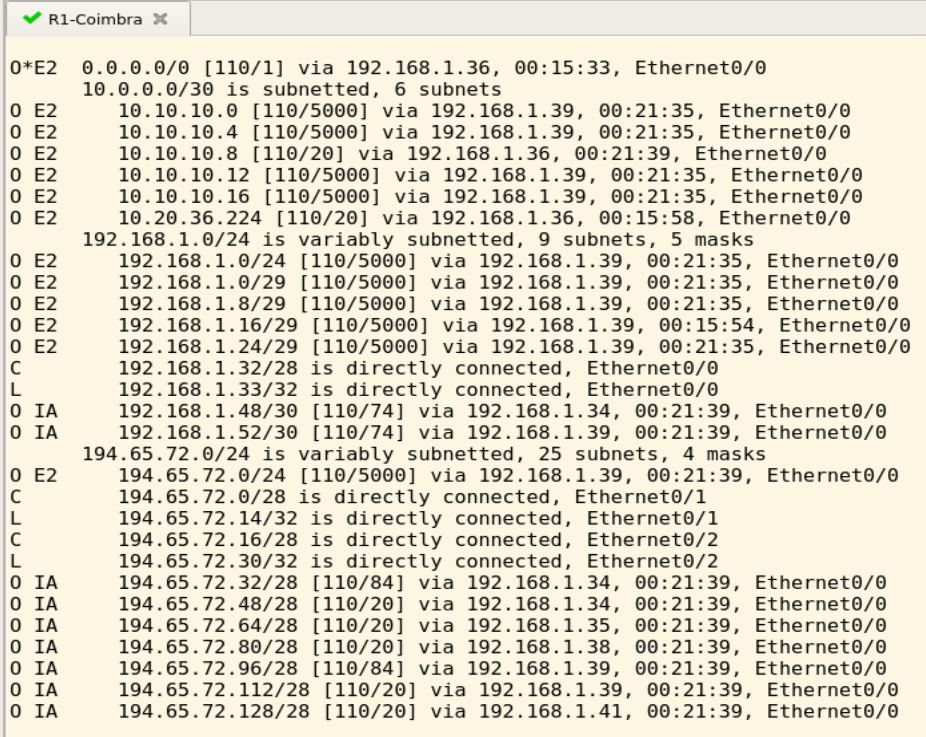
\includegraphics[width=0.6\textwidth]{routing-coimbra}
		\caption{Excerto da tabela de \emph{routing} de Coimbra}
		\label{fig.nav}
	\end{figure}

	\pagebreak 

	\begin{figure}[h]
		\centering
		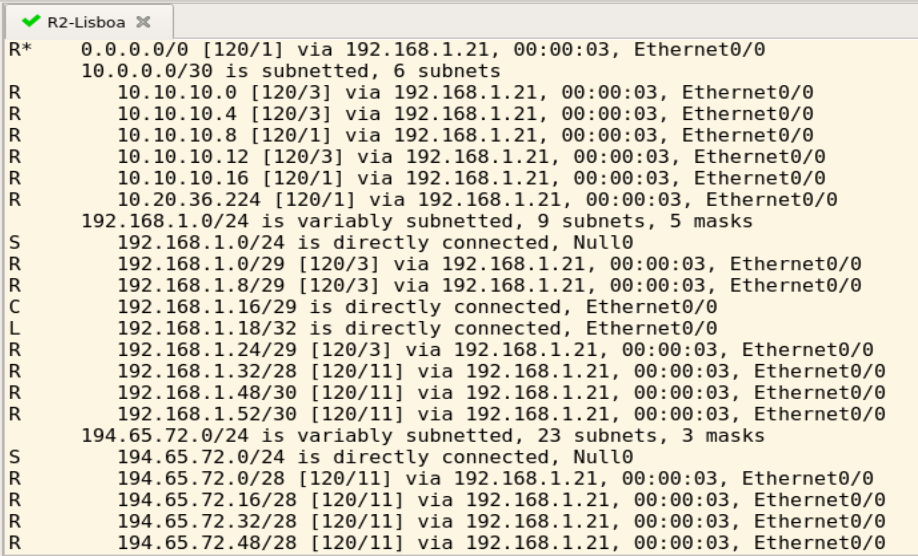
\includegraphics[width=0.7\textwidth]{routing-lisboa}
		\caption{Excerto da tabela de \emph{routing} de Lisboa}
		\label{fig.nav}
	\end{figure}
	

    \pagebreak
	\large
	\section{Conclusão}
	\normalsize
	\paragraph{}
	No fim todos os objetivos propostos no enunciado do trabalho foram conseguidos fazendo com que fossem aplicados todos os conhecimentos e técnicas aprendidas e praticadas tanto nas aulas práticas como nas aulas teóricas da cadeira de encaminhamento de dados.

\end{document}